\documentclass[tikz,border=4pt]{standalone}
\usepackage{tikz}
\usepackage{polymer-paper-preamble}
\usetikzlibrary{arrows.meta,calc,decorations.pathmorphing,positioning}

\begin{document}
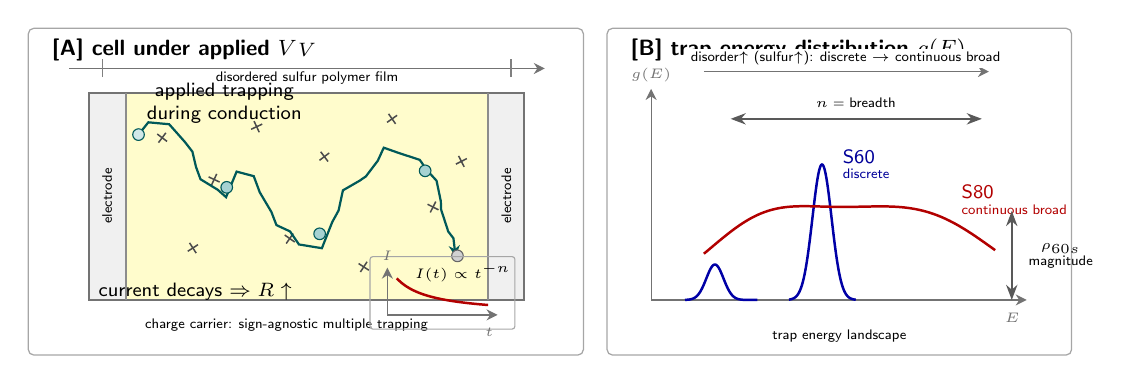
\begin{tikzpicture}[
  font=\sffamily,
  >=Stealth,
  panel/.style={draw=black!35, line width=0.45pt, rounded corners=2pt},
  title/.style={font=\sffamily\bfseries\footnotesize, anchor=west},
  tinylabel/.style={font=\sffamily\scriptsize, align=center},
  note/.style={font=\sffamily\tiny, align=center},
  carrier/.style={circle, draw=teal!70!black, fill=teal!18, minimum size=4.2pt, inner sep=0pt},
  trap/.style={black!70, line width=0.55pt},
  flow/.style={teal!70!black, line width=0.8pt, -{Stealth[length=4pt,width=4pt]}},
  axis/.style={black!55, line width=0.45pt, -{Stealth[length=4pt,width=4pt]}},
  curve/.style={line width=0.9pt}
]

% Canvas panels: slim, dense schematic half.
\draw[panel] (0,0) rectangle (7.05,4.15);
\draw[panel] (7.35,0) rectangle (13.25,4.15);

% Panel labels and titles.
\node[title] at (0.18,3.88) {[A] cell under applied $V$};
\node[title] at (7.53,3.88) {[B] trap-energy distribution $g(E)$};

% --------------------------------------------------------------------------
% A. Applied voltage cell, dispersive repeated trapping, current decay.
% --------------------------------------------------------------------------
\begin{scope}[shift={(0.22,0.18)}]
  % Cell body.
  \fill[gray!12] (0.55,0.52) rectangle (1.02,3.15);
  \fill[yellow!20] (1.02,0.52) rectangle (5.62,3.15);
  \fill[gray!12] (5.62,0.52) rectangle (6.08,3.15);
  \draw[black!55,line width=0.65pt] (0.55,0.52) rectangle (6.08,3.15);
  \draw[black!45,line width=0.55pt] (1.02,0.52) -- (1.02,3.15);
  \draw[black!45,line width=0.55pt] (5.62,0.52) -- (5.62,3.15);
  \node[note, rotate=90] at (0.78,1.84) {electrode};
  \node[note, rotate=90] at (5.85,1.84) {electrode};
  \node[note] at (3.32,3.34) {disordered sulfur polymer film};

  % Applied V fixture; placed away from transport phrase.
  \draw[axis] (0.30,3.46) -- (6.34,3.46);
  \node[tinylabel, anchor=south] at (3.32,3.49) {$V$};
  \draw[black!50] (0.72,3.35) -- (0.72,3.58);
  \draw[black!50] (5.91,3.35) -- (5.91,3.58);

  % Unlabeled trap-site crosses.
  \foreach \x/\y/\r in {
    1.48/2.58/8, 1.87/1.18/-12, 2.14/2.05/20, 2.68/2.72/-20,
    3.10/1.30/10, 3.54/2.34/-8, 4.04/0.94/12, 4.40/2.82/-10,
    4.92/1.70/18, 5.28/2.28/-18}
  {
    \begin{scope}[shift={(\x,\y)}, rotate=\r]
      \draw[trap] (-0.055,-0.055) -- (0.055,0.055);
      \draw[trap] (-0.055,0.055) -- (0.055,-0.055);
    \end{scope}
  }

  % Sign-agnostic carrier walk with repeated trapping; not a clean drift band.
  \draw[flow, decorate, decoration={random steps, segment length=5.5pt, amplitude=2.0pt}]
    (1.18,2.62) .. controls (1.80,3.03) and (2.03,1.62) .. (2.30,1.95)
    .. controls (2.67,2.48) and (3.10,0.82) .. (3.48,1.36)
    .. controls (3.92,1.98) and (4.36,2.82) .. (4.82,2.16)
    .. controls (5.08,1.80) and (5.10,1.23) .. (5.23,1.08);
  \node[carrier] at (1.18,2.62) {};
  \node[carrier, fill=teal!35] at (2.30,1.95) {};
  \node[carrier, fill=teal!35] at (3.48,1.36) {};
  \node[carrier, fill=teal!35] at (4.82,2.16) {};
  \node[carrier, fill=black!18, draw=black!60] at (5.23,1.08) {};
  \node[note, anchor=west] at (1.14,0.20) {charge carrier: sign-agnostic multiple trapping};

  % Clearance-sensitive text group, separated from V label above.
  \node[tinylabel, anchor=west, text width=2.25cm] at (1.02,3.02)
    {applied trapping during conduction};

  % Current decay inset.
  \begin{scope}[shift={(4.12,0.15)}]
    \draw[black!35, rounded corners=1pt] (0,0) rectangle (1.84,0.92);
    \draw[axis] (0.22,0.18) -- (1.62,0.18) node[below left=1pt and -2pt, font=\tiny] {$t$};
    \draw[axis] (0.22,0.18) -- (0.22,0.78) node[above=-1pt, font=\tiny] {$I$};
    \draw[curve, red!70!black, domain=0.06:1.22, samples=80]
      plot ({0.28+\x}, {0.18+0.54/(1+2.7*\x)});
    \node[note, anchor=west] at (0.45,0.72) {$I(t)\propto t^{-n}$};
  \end{scope}
  \node[tinylabel, anchor=west] at (0.55,0.62) {current decays $\Rightarrow R\uparrow$};
\end{scope}

% --------------------------------------------------------------------------
% B. Distribution evolution: breadth n, magnitude rho60s.
% --------------------------------------------------------------------------
\begin{scope}[shift={(7.56,0.28)}]
  \draw[axis] (0.35,0.42) -- (5.12,0.42) node[below left=1pt and -1pt, font=\tiny] {$E$};
  \draw[axis] (0.35,0.42) -- (0.35,3.10) node[above=-1pt, font=\tiny] {$g(E)$};
  \node[note, anchor=north] at (2.74,0.16) {trap energy landscape};

  % S60: discrete narrow deep feature, plus faint shallow marker without asserting all compositions fixed.
  \draw[curve, blue!65!black, domain=0.78:1.70, samples=70]
    plot (\x, {0.42 + 0.45*exp(-42*(\x-1.16)^2)});
  \draw[curve, blue!65!black, domain=2.10:2.95, samples=90]
    plot (\x, {0.42 + 1.72*exp(-34*(\x-2.52)^2)});
  \node[tinylabel, blue!60!black, anchor=west] at (2.66,2.24) {S60};
  \node[note, blue!60!black, anchor=west] at (2.66,2.02) {discrete};

  % S80: continuous broad distribution.
  \draw[curve, red!70!black, domain=1.02:4.72, samples=110]
    plot (\x, {0.42 + 0.55*exp(-1.1*(\x-1.65)^2)
                    + 1.02*exp(-0.36*(\x-3.05)^2)
                    + 0.34*exp(-0.95*(\x-4.18)^2)});
  \node[tinylabel, red!70!black, anchor=west] at (4.17,1.79) {S80};
  \node[note, red!70!black, anchor=west] at (4.17,1.57) {continuous broad};

  % Breadth and magnitude annotations: separate semantics.
  \draw[<->, black!65, line width=0.55pt] (1.36,2.72) -- (4.55,2.72);
  \node[note, fill=white, inner sep=1pt] at (2.95,2.92) {$n$ = breadth};

  \draw[<->, black!65, line width=0.55pt] (4.93,0.42) -- (4.93,1.55);
  \node[note, anchor=west] at (5.02,0.98) {$\rho_{60s}$\\magnitude};

  \draw[-{Stealth[length=4pt,width=4pt]}, black!55, line width=0.55pt]
    (1.02,3.32) -- (4.64,3.32);
  \node[note, fill=white, inner sep=1pt] at (2.82,3.49)
    {disorder$\uparrow$ (sulfur$\uparrow$): discrete $\rightarrow$ continuous broad};
\end{scope}

\end{tikzpicture}
\end{document}
